\documentclass{article}\usepackage[]{graphicx}\usepackage[]{color}
%% maxwidth is the original width if it is less than linewidth
%% otherwise use linewidth (to make sure the graphics do not exceed the margin)
\makeatletter
\def\maxwidth{ %
  \ifdim\Gin@nat@width>\linewidth
    \linewidth
  \else
    \Gin@nat@width
  \fi
}
\makeatother

\definecolor{fgcolor}{rgb}{0.345, 0.345, 0.345}
\newcommand{\hlnum}[1]{\textcolor[rgb]{0.686,0.059,0.569}{#1}}%
\newcommand{\hlstr}[1]{\textcolor[rgb]{0.192,0.494,0.8}{#1}}%
\newcommand{\hlcom}[1]{\textcolor[rgb]{0.678,0.584,0.686}{\textit{#1}}}%
\newcommand{\hlopt}[1]{\textcolor[rgb]{0,0,0}{#1}}%
\newcommand{\hlstd}[1]{\textcolor[rgb]{0.345,0.345,0.345}{#1}}%
\newcommand{\hlkwa}[1]{\textcolor[rgb]{0.161,0.373,0.58}{\textbf{#1}}}%
\newcommand{\hlkwb}[1]{\textcolor[rgb]{0.69,0.353,0.396}{#1}}%
\newcommand{\hlkwc}[1]{\textcolor[rgb]{0.333,0.667,0.333}{#1}}%
\newcommand{\hlkwd}[1]{\textcolor[rgb]{0.737,0.353,0.396}{\textbf{#1}}}%

\usepackage{framed}
\makeatletter
\newenvironment{kframe}{%
 \def\at@end@of@kframe{}%
 \ifinner\ifhmode%
  \def\at@end@of@kframe{\end{minipage}}%
  \begin{minipage}{\columnwidth}%
 \fi\fi%
 \def\FrameCommand##1{\hskip\@totalleftmargin \hskip-\fboxsep
 \colorbox{shadecolor}{##1}\hskip-\fboxsep
     % There is no \\@totalrightmargin, so:
     \hskip-\linewidth \hskip-\@totalleftmargin \hskip\columnwidth}%
 \MakeFramed {\advance\hsize-\width
   \@totalleftmargin\z@ \linewidth\hsize
   \@setminipage}}%
 {\par\unskip\endMakeFramed%
 \at@end@of@kframe}
\makeatother

\definecolor{shadecolor}{rgb}{.97, .97, .97}
\definecolor{messagecolor}{rgb}{0, 0, 0}
\definecolor{warningcolor}{rgb}{1, 0, 1}
\definecolor{errorcolor}{rgb}{1, 0, 0}
\newenvironment{knitrout}{}{} % an empty environment to be redefined in TeX

\usepackage{alltt}
\usepackage{amscd, amssymb, amsmath, verbatim, setspace}
\usepackage[left=1.0in, right=1.0in, top=1.0in, bottom=1.0in]{geometry}
\usepackage{mathrsfs}
\usepackage{listings}


\IfFileExists{upquote.sty}{\usepackage{upquote}}{}
\begin{document}

\begin{flushright}
  Arif Ali\\
  ANLY-511 Prob. Modeling \& Stat. Computing\\
	Oct 29, 2015\\
\end{flushright}

\begin{center}
  \LARGE\textbf{Homework \#6}
\end{center}

\section*{Problem 41}
\begin{knitrout}
\definecolor{shadecolor}{rgb}{1, 1, 1}\color{fgcolor}\begin{kframe}
\begin{verbatim}
Z = (51-48)/(9/sqrt(30))
pnorm(Z, lower.tail = F)
## [1] 0.03394458
\end{verbatim}
\end{kframe}
\end{knitrout}
\section*{Problem 42}
For each Xi ~ U(0,1) the mean is .5 so the mean of Z is 12*.5-6 = 0. For the variance of each Xi, it is 1/12*(1-0) = 1/12. The Variance of Z is 1/12*12 - 0 = 1. Z has the mean and variance of a standard normal distribution. By theorem 4.2, since all X are i.i.d witht the same variances and means, then any constant z will follow the normal distribution.
\section*{Problem 43}
\subsection*{Part A}
\begin{knitrout}
\definecolor{shadecolor}{rgb}{1, 1, 1}\color{fgcolor}\begin{kframe}
\begin{verbatim}
#Part A
meanY_X = 7-10
#[1] -3
sdY_X = sqrt(9/sqrt(9)+25/sqrt(12))
#[1] 3.196385
\end{verbatim}
\end{kframe}
\end{knitrout}
\subsection*{Part B}
\begin{knitrout}
\definecolor{shadecolor}{rgb}{1, 1, 1}\color{fgcolor}\begin{kframe}
\begin{verbatim}
simX_Y = function(i){
  X = rnorm(9, mean = 7, sd = 3)
  Y = rnorm(12, mean = 10, sd = 5)
  meanY_X = mean(X) - mean(Y)
  sdY_X = sqrt((sd(X))^2/sqrt(length(X))+(sd(Y))^2/sqrt(length(Y)))
  return(list(meanY_X, sdY_X))
}
Problem43B = sapply(1:10000, simX_Y)

Problem43B = as.data.frame(t(Problem43B))
par(mfrow = c(1,2))
hist(unlist(Problem43B$V1), breaks = 25)
abline(v = meanY_X, col = "red", lwd = 2)
mean(unlist(Problem43B$V1))
## [1] -2.979591
hist(unlist(Problem43B$V2), breaks = 25)
abline(v = sdY_X, col = "red", lwd = 2)
\end{verbatim}
\end{kframe}
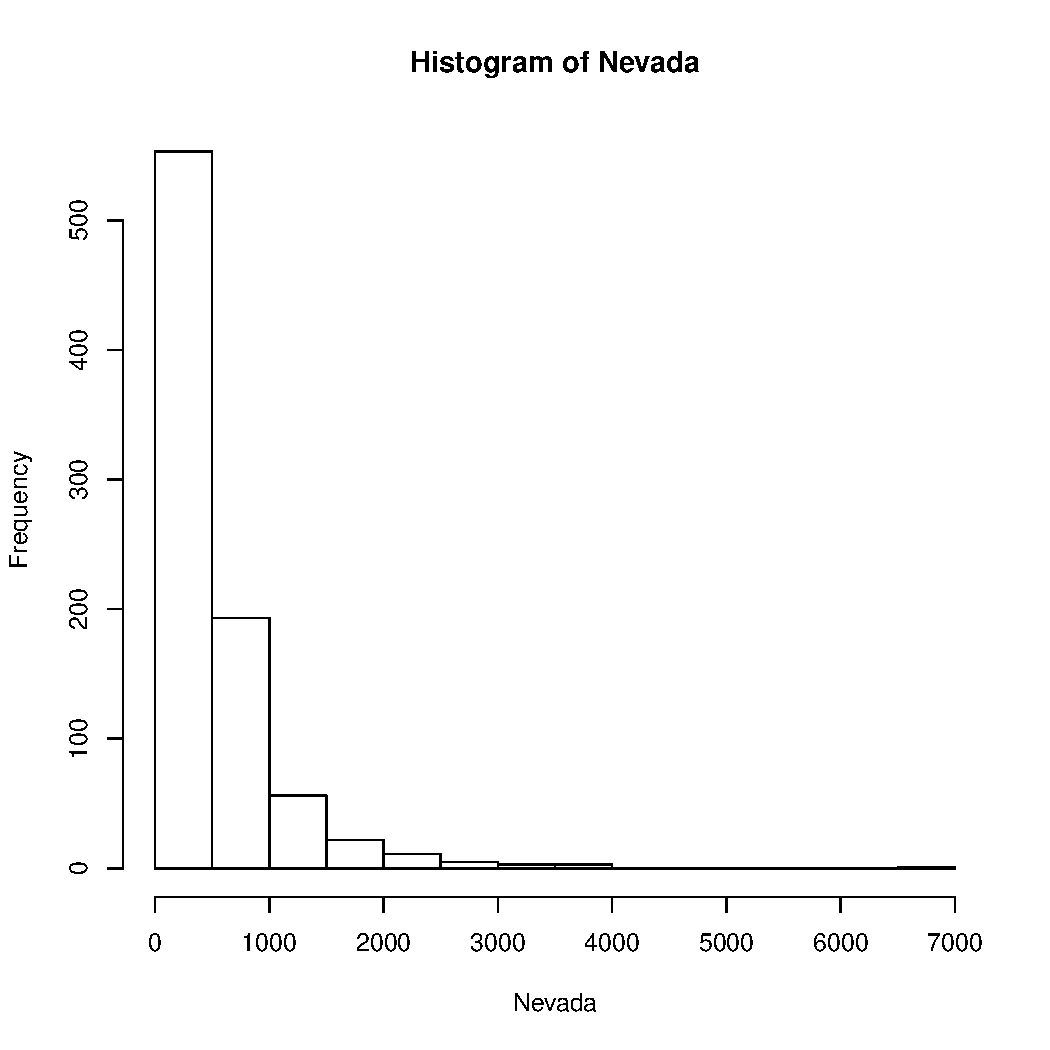
\includegraphics[width=0.33\linewidth]{figure/unnamed-chunk-4-1} 
\begin{kframe}\begin{verbatim}
mean(unlist(Problem43B$V2))
## [1] 3.157558
\end{verbatim}
\end{kframe}
\end{knitrout}
Based on the histogram and the means of the simulationed SE and mean, both seem close to the theoretical ones.
\section*{Problem 44}
\subsection*{Part A}
\begin{knitrout}
\definecolor{shadecolor}{rgb}{1, 1, 1}\color{fgcolor}\begin{kframe}
\begin{verbatim}
X20 = replicate(1000, sum(rexp(20, rate = 2)))
hist(X20, probability = T, breaks = 25)
\end{verbatim}
\end{kframe}
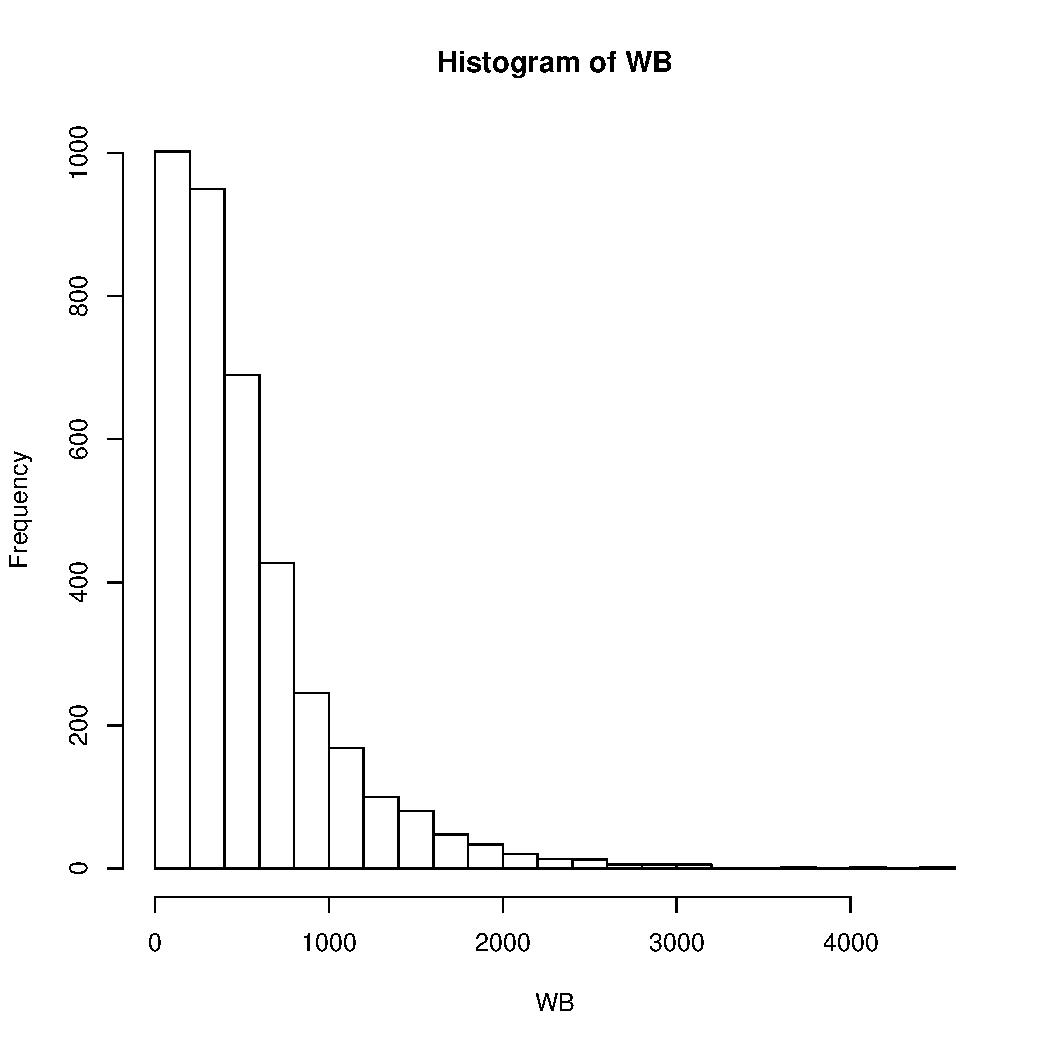
\includegraphics[width=0.33\linewidth]{figure/unnamed-chunk-5-1} 

\end{knitrout}
\subsection*{Part B}
\begin{knitrout}
\definecolor{shadecolor}{rgb}{1, 1, 1}\color{fgcolor}\begin{kframe}
\begin{verbatim}
mean(X20)
## [1] 9.935507
var(X20)
## [1] 4.639166
\end{verbatim}
\end{kframe}
\end{knitrout}
\subsection*{Part C}
\begin{knitrout}
\definecolor{shadecolor}{rgb}{1, 1, 1}\color{fgcolor}\begin{kframe}
\begin{verbatim}
mean(X20<=10)
## [1] 0.54
\end{verbatim}
\end{kframe}
\end{knitrout}
\section*{Problem 45}
\begin{knitrout}
\definecolor{shadecolor}{rgb}{1, 1, 1}\color{fgcolor}\begin{kframe}
\begin{verbatim}
par(mfrow = c(1,2))
my.vars = sapply(rep(20, times = 1000), function(x){var(rnorm(x, 25, 7))})
mean(my.vars)
## [1] 49.25078
var(my.vars)
## [1] 253.393
hist(my.vars, breaks = 25)
#dev.new()
qqnorm(my.vars)
qqline(my.vars)
\end{verbatim}
\end{kframe}
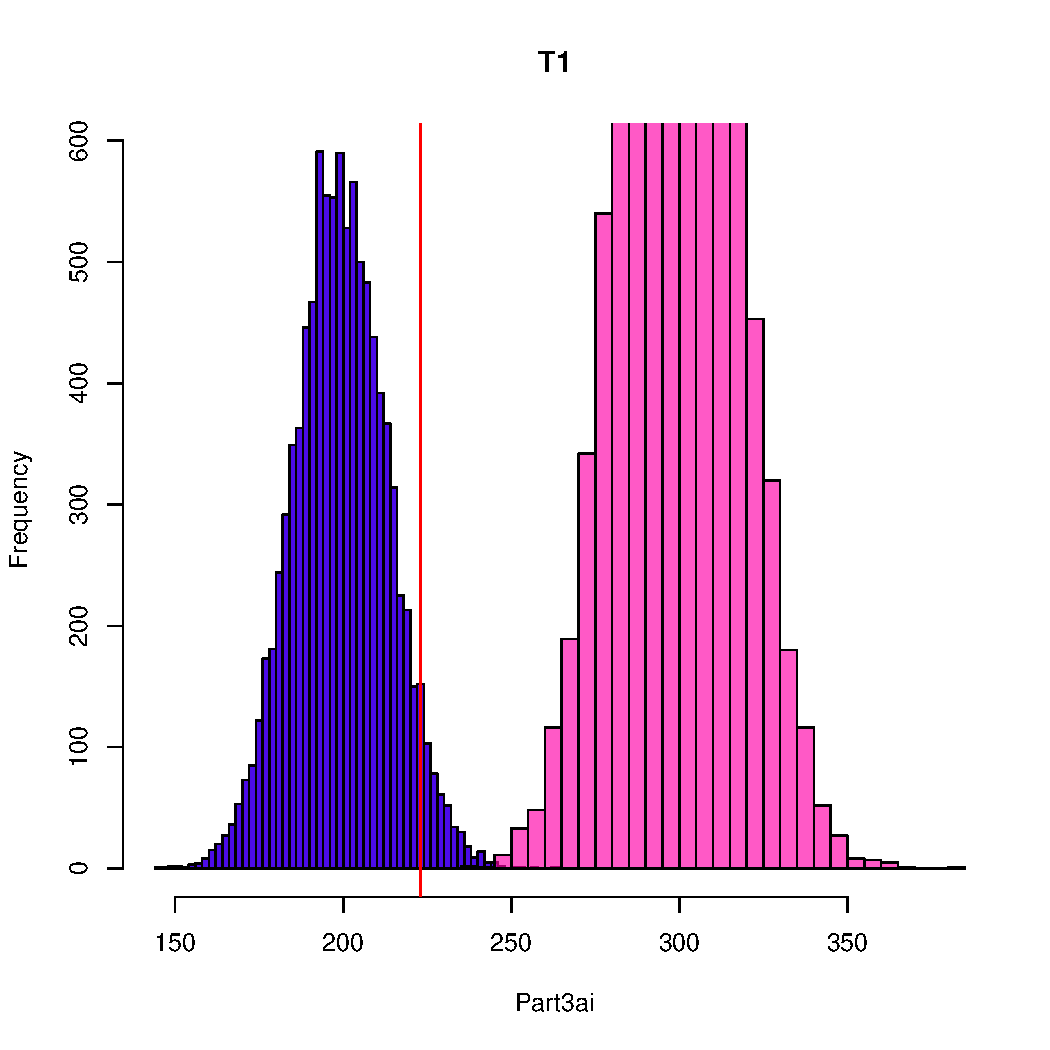
\includegraphics[width=0.33\linewidth]{figure/unnamed-chunk-8-1} 

\end{knitrout}
At n = 20, the qqnorm plot does not follow the the qqline; therefore, it does not appear to be normally distributed. The Histogram is skrewed
\begin{knitrout}
\definecolor{shadecolor}{rgb}{1, 1, 1}\color{fgcolor}\begin{kframe}
\begin{verbatim}
par(mfrow = c(1,2))
my.vars = sapply(rep(50, times = 1000), function(x){var(rnorm(x, 25, 7))})
mean(my.vars)
## [1] 48.85999
var(my.vars)
## [1] 102.7943
hist(my.vars, breaks = 25)
#dev.new()
qqnorm(my.vars)
qqline(my.vars)
\end{verbatim}
\end{kframe}
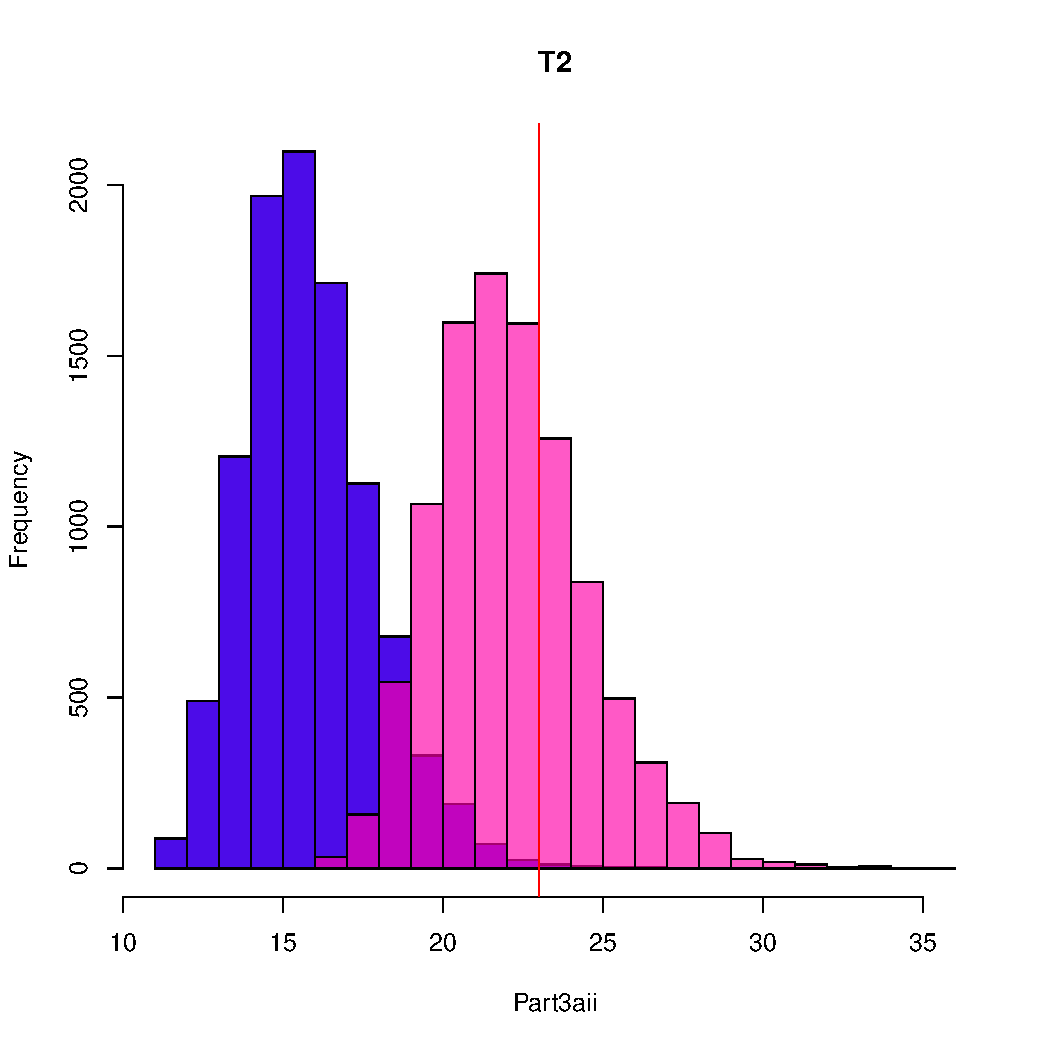
\includegraphics[width=0.33\linewidth]{figure/unnamed-chunk-9-1} 

\end{knitrout}
At n = 50, the qqnorm plot follows the qqline close than at n = 20, but it still deviates a significant amount of the time so, it does not appear to be normally distributed. The histogram has two peaks.
\begin{knitrout}
\definecolor{shadecolor}{rgb}{1, 1, 1}\color{fgcolor}\begin{kframe}
\begin{verbatim}
par(mfrow = c(1,2))
my.vars = sapply(rep(200, times = 1000), function(x){var(rnorm(x, 25, 7))})
mean(my.vars)
## [1] 49.00263
var(my.vars)
## [1] 22.51143
hist(my.vars, breaks = 25)
#dev.new()
qqnorm(my.vars)
qqline(my.vars)
\end{verbatim}
\end{kframe}
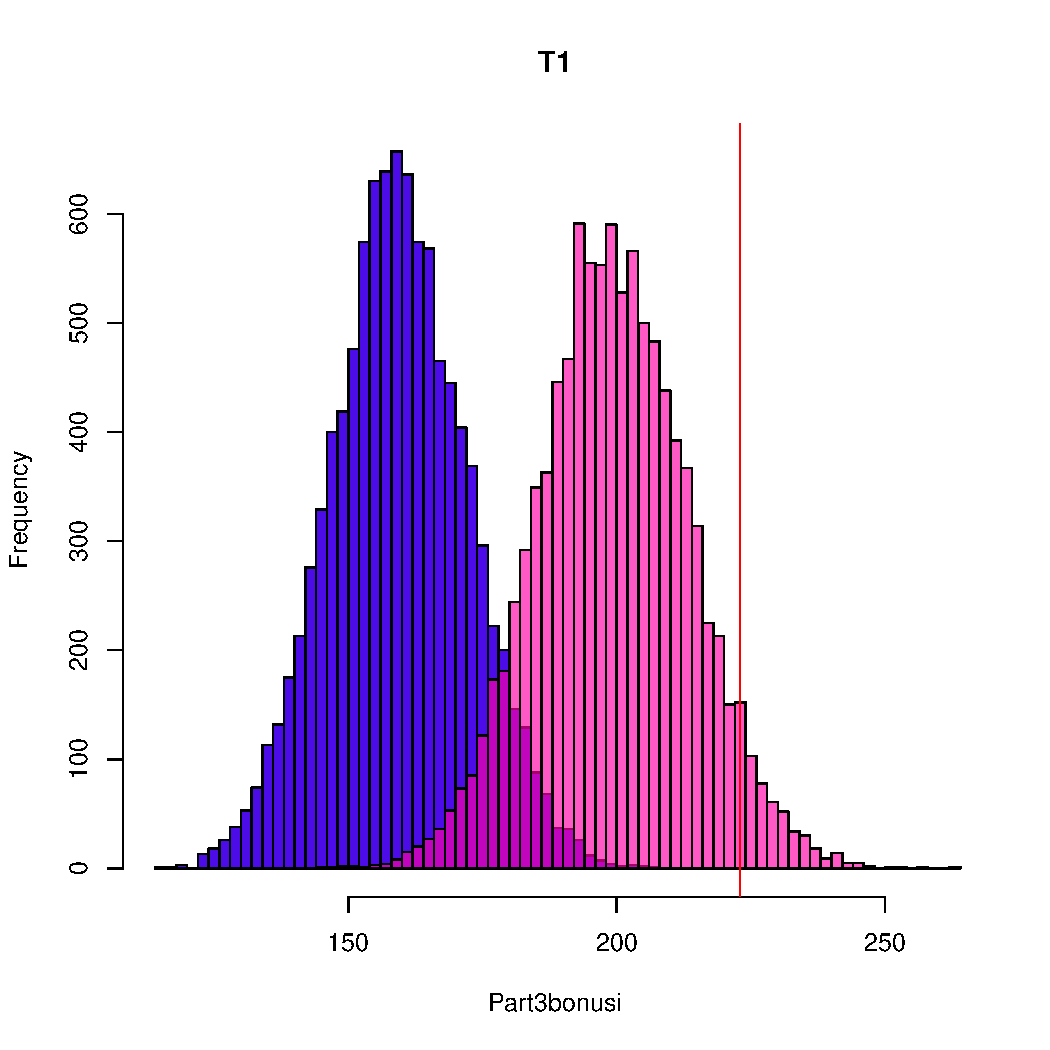
\includegraphics[width=0.33\linewidth]{figure/unnamed-chunk-10-1} 

\end{knitrout}
At n = 200, it closely follows the line so it is normally distributed. The histogram is a rough, but looks somewaht bell shaped.
\section*{Problem 46}
\begin{knitrout}
\definecolor{shadecolor}{rgb}{1, 1, 1}\color{fgcolor}\begin{kframe}
\begin{verbatim}
pop = c(3,6,7,9,11,14)
Problem46 = combn(pop, m = 3, FUN = min)
mean(Problem46)
## [1] 4.8
hist(Problem46)
\end{verbatim}
\end{kframe}
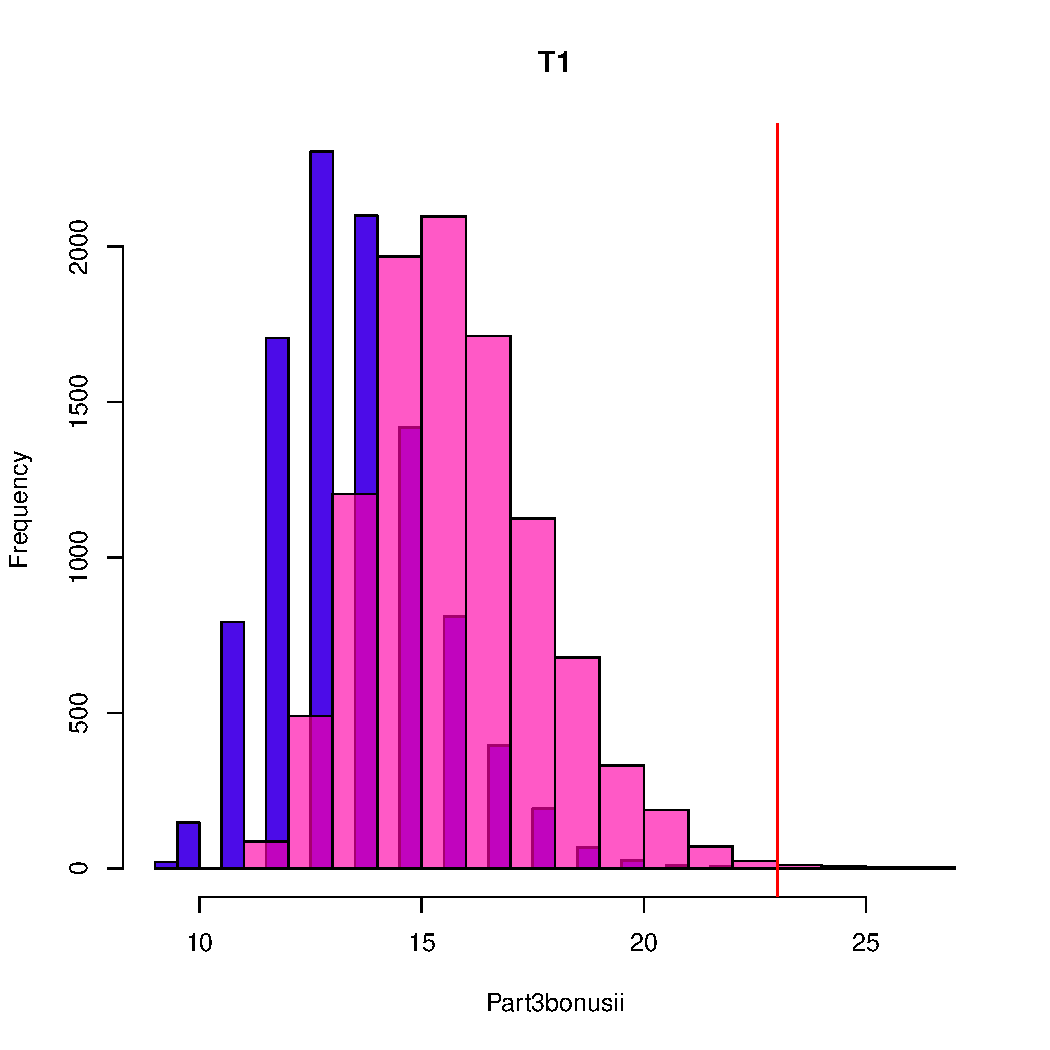
\includegraphics[width=0.33\linewidth]{figure/unnamed-chunk-11-1} 

\end{knitrout}
It looks like we are trying to estimate the min of the population. That seems to be the parameter we are trying to find.
\section*{Problem 47}
\subsection*{Part A}
\begin{equation*}
E(X)=10
\end{equation*}
\subsection*{Part B}
\begin{knitrout}
\definecolor{shadecolor}{rgb}{1, 1, 1}\color{fgcolor}\begin{kframe}
\begin{verbatim}
my.means = replicate(1000, mean(rexp(30, rate = 1/10)))
mean(my.means>=12)
## [1] 0.15
\end{verbatim}
\end{kframe}
\end{knitrout}
\subsection*{Part C}
The proportion doesn't seem too small, so it doesn't seem to be unusual.
\section*{Problem 48}
\subsection*{Part A}
\begin{equation*}
f_{min}(x)=n(1-(1-e^{-\lambda x}))^{n-1}*\lambda e^{-\lambda x}=n*e^{(n-1)-\lambda x}*\lambda^{-\lambda x}=n\lambda e^{-n\lambda}
\end{equation*} 
\begin{equation*}
\therefore X_{min}\sim Exp(n\lambda)
\end{equation*}
\subsection*{Part B}
\begin{knitrout}
\definecolor{shadecolor}{rgb}{1, 1, 1}\color{fgcolor}\begin{kframe}
\begin{verbatim}
Problem48B = replicate(1000, min(rexp(25, rate = 7)))
1/(25*7) - mean(Problem48B)
## [1] -0.000425932
\end{verbatim}
\end{kframe}
\end{knitrout}
\end{document}
